\documentclass{article}
\usepackage[utf8]{inputenc}

\title{Written Assignment 1}
\author{Benny Chen}
\date{\today}

\usepackage{color}
\usepackage{amsthm}
\usepackage{amssymb} 
\usepackage{amsmath}
\usepackage{listings}
\usepackage{xcolor}
\usepackage{listings}
\usepackage{graphicx}
\usepackage[hidelinks]{hyperref}

\definecolor{codegreen}{rgb}{0,0.6,0}
\definecolor{codegray}{rgb}{0.5,0.5,0.5}
\definecolor{codepurple}{rgb}{0.58,0,0.82}
\definecolor{backcolour}{rgb}{0.95,0.95,0.92}

\lstdefinestyle{mystyle}{
    backgroundcolor=\color{backcolour},   
    commentstyle=\color{codegreen},
    keywordstyle=\color{magenta},
    numberstyle=\tiny\color{codegray},
    stringstyle=\color{codepurple},
    basicstyle=\ttfamily\footnotesize,
    breakatwhitespace=false,         
    breaklines=true,                 
    captionpos=b,                    
    keepspaces=true,                 
    numbers=left,                    
    numbersep=5pt,                  
    showspaces=false,                
    showstringspaces=false,
    showtabs=false,                  
    tabsize=2
}

\lstset{style=mystyle}

\begin{document}

\maketitle

\section{Data Preprocessing}



\subsection*{Classify the following attributes as binary, discrete, or continuous. Also classify them as qualitative (nominal or ordinal) or quantitative (interval or ratio). Some cases may have more than one interpretation, so briefly indicate your reasoning if you think there may be some ambiguity.}

\begin{enumerate}
    \item Seat numbers assigned to passengers on a flight.
    \item Hurricane intensity measured on the Saffir-Simpson scale.
    \item Social Security number.
\end{enumerate}

\begin{enumerate}
    \item The seat numbers assigned to passengers on a flight would be a discrete attribute as there is only a finite number of seats on a plane and can only be integer values. This attribute would also be a qualitative attribute, specifically a ordinal attribute as the seat numbers are ordered from the first sear and passenger to the last seat and passenger.
    \item Hurricane intensity measured on the Saffir-Simpson scale would also be a discrete attribute as there is only a finite number of categories on the scale and each category is a integer value scaled from 1 to 5. This attribute would also be a qualitative attribute, specifically a ordinal attribute as the categories are ordered from the lowest intensity to the highest intensity.
    \item This prompt is very ambiguous as we don't know what we are supposed to do with the Social Security number. If we are supposed to use the Social Security number as an attribute, then it would be a discrete attribute as there is only a finite number of Social Security numbers that there can be in total. This attribute would also be a qualitative attribute, specifically a nominal attribute as the Social Security numbers are not ordered and are a categorical attribute.
\end{enumerate}

\subsection*{Consider the following binary vectors:}
\[x_1 = (1,1,1,1,1)\]
\[x_2 = (1,1,1,0,0)\]
\[y_1 = (0,0,0,0,0)\]
\[y_2 = (0,0,0,1,1)\]

\begin{enumerate}
    \item According to the Jaccard coefficient, which pair of vectors ($x_1$; $x_2$) or ($y_1$; $y_2$) are more similar to each other?
    \item According to the Simple Matching proximity measure, which pair of vectors ($x_1$; $x_2$) or ($y_1$; $y_2$) are more similar to each other?
    \item According to the Euclidean Distance, which pair of vectors ($x_1$; $x_2$) or ($y_1$; $y_2$) are more similar to each other?
\end{enumerate}

\begin{enumerate}
    \item The Jaccard coefficient is used to find similarities between 2 sets which is \[sim_{Jaccard}(i,j) = \frac{q}{q+r+s}\] We first create a contingency table of 
    \begin{table}[h]
        \begin{tabular}{|l|l|l|l|}
        \hline
        X1/X2 & 1 & 0 & Sum \\ \hline
        1 & 3 & 0 & 3 \\ \hline
        0 & 2 & 0 & 2 \\ \hline
        Sum & 5 & 0 & 5 \\ \hline
        \end{tabular}
        \centering
    \end{table} 
    then plug in the values for each set and find that the pair of vectors ($x_1$; $x_2$) are 3/5 or 60\% similar to each other. The pair of vectors ($y_1$; $y_2$) are 0/2 or 0\% similar to each other. Therefore, the pair of vectors ($x_1$; $x_2$) are more similar to each other.
    \item We can use simple matching which is \[d(i,j) = \frac{p - m}{p}\]
    to find for that both pairs of vectors ($x_1$; $x_2$) and ($y_1$; $y_2$) 60\% similar to each other as we are finding the number of matches regardless of the value.
    \item According to the Euclidean Distance, both pairs of vectors are similar to each other. The Euclidean Distance is \[d(i,j) = \sqrt{\sum_{k=1}^n (x_k - y_k)^2}\] We then plug in the values for each set and find that the pair of vectors ($x_1$; $x_2$) to get \[d(x_1,x_2) = \sqrt{(1-1)^2 + (1-1)^2 + (1-1)^2 + (1-0)^2 + (1-0)^2} = \sqrt{2}\] and the pair of vectors ($y_1$; $y_2$) to get \[d(y_1,y_2) = \sqrt{(0-0)^2 + (0-0)^2 + (0-0)^2 + (0-1)^2 + (0-1)^2} = \sqrt{2}\] Therefore, both pairs of vectors are similar to each other.
\end{enumerate}

\subsection*{We are given the traffic accident of three drivers. We consider the three attributes are asymmetric binary ones, i.e., ``Alcohol Impaired = Yes", ``Traffic Violation = Yes". , and ``Absence of Belt = Yes" are more severe/critical. Please find their respective similarity based on contingency tables and Distance Measure for Asymmetric Binary Variables.}

\begin{table}[h]
    \begin{tabular}{|l|l|l|l|}
    \hline
    Driver & Alcohol Impaired & Traffic Violation & Absence of Belt \\ \hline
    Han    & Yes              & Yes               & Yes             \\ \hline
    Luke   & No               & No                & Yes             \\ \hline
    Leia   & No               & Yes               & No              \\ \hline
    \end{tabular}
    \centering
\end{table}

\noindent
To find the Distance Measure for Asymmetric Variables and the similarities between the three people, we need a contingency table for each pair of people. We then use the following formula to find the similarity between the two people. \[dis_{Asymmetric}(i,j) = \frac{r+s}{q+r+s}\] 
\noindent
For the contingency table for Luke (Column) and Han (Row) we will get:

\begin{table}[h]
    \begin{tabular}{|l|l|l|l|}
    \hline
    Luke/Han & 1 & 0 & Sum \\ \hline
    1 & 1 & 0 & 1 \\ \hline
    0 & 2 & 0 & 2 \\ \hline
    Sum & 3 & 0 & 3 \\ \hline
    \end{tabular}
    \centering
\end{table}

\[\frac{0 + 2}{1 + 0 + 2} = 0.67\]

\noindent
The contingency table for Luke (Column) and Lelia (Row) will get us:

\begin{table}[h]
    \begin{tabular}{|l|l|l|l|}
    \hline
    Luke/Lelia & 1 & 0 & Sum \\ \hline
    1 & 0 & 1 & 1 \\ \hline
    0 & 1 & 1 & 2 \\ \hline
    Sum & 1 & 2 & 3 \\ \hline
    \end{tabular}
    \centering
\end{table}

\[\frac{1 + 1}{0 + 1 + 1} = 1\]

\noindent
\newpage
Lastly the contingency table for Leila (Column) and Han (Row):

\begin{table}[h]
    \begin{tabular}{|l|l|l|l|}
    \hline
    Lelia/Han & 1 & 0 & Sum \\ \hline
    1 & 1 & 0 & 1 \\ \hline
    0 & 2 & 0 & 2 \\ \hline
    Sum & 3 & 0 & 3 \\ \hline
    \end{tabular}
    \centering
\end{table}

\[\frac{0 + 2}{1 + 0 + 2} = 0.67\]
\noindent
From what we can see, the similarity between Luke and Leia is 1 while the similarity between Luke and Han and Leia and Han is 0.67. This means that the pair of Luke and Han and Leia and Han are more similar to each other than Luke and Leia.

\section{Association Rule Mining}

\subsection*{Frequent Pattern Mining}

Please determine whether the statement is true or false and provide your explanation.

\begin{enumerate}
    \item For some transaction data, the number of frequent itemsets of size 3 was found out to be three. Is it safe to assume that there cannot be any frequent itemset of size 4? If no, come up with an example. If yes, justify your answer.
    \item Given that \{a,b\}, \{b,c\} and \{a,c\} are frequent itemsets, \{a,b,c\} is always frequent.
\end{enumerate}

\begin{enumerate}
    \item This statement is false that we can assume that there cannot be any frequent itemset of size 4 since there is a frequent itemset of size 3. We cannot assume that there will always be 3 as the size could change due to any factor and could find frequent itemsets of 4. For example a frequent itemset of size 4 could be \{a,b,c,d\}, \{a,b,c,e\}, and \{a,b,c,f\} but also have a frequent itemset of size 3 with \{a,b,c\} as the subsets of the frequent itemsets of size 4. 
    \item This statement is True as subsets of frequent itemsets would make a frequent itemset. \{a,b\}, \{b,c\}, and \{a,c\} are subsets of \{a,b,c\}. Therefore, \{a,b,c\} is always frequent.
\end{enumerate}
\newpage
\subsection*{FP-Tree}
We are given the transaction database as:

\begin{table}[h]
    \begin{tabular}{|l|l|}
    \hline
    TID & Item Bought \\ \hline
    T1  & A,C,D       \\ \hline
    T2  & A,B,C       \\ \hline
    T3  & A,B,E       \\ \hline
    T4  & B,E         \\ \hline
    \end{tabular}
    \centering
\end{table}

\noindent
Please build the FPTree for the transaction database with the minimum support count 2. Please provide clear and readable figure or screenshot of the constructed FPTree (refer to the lecture note). We assume alphabetical order for items with the same frequency. You do not need to build the conditional FPTrees and the rules.
\\\noindent
We first need to count and order all the items by frequency. From that we can tell A and B are the most frequent, followed by C and E with 2 and finally D with 1. We then filter out the items that do not meet the minimum support count of 2 then we build the tree to get the following:

\begin{center}
    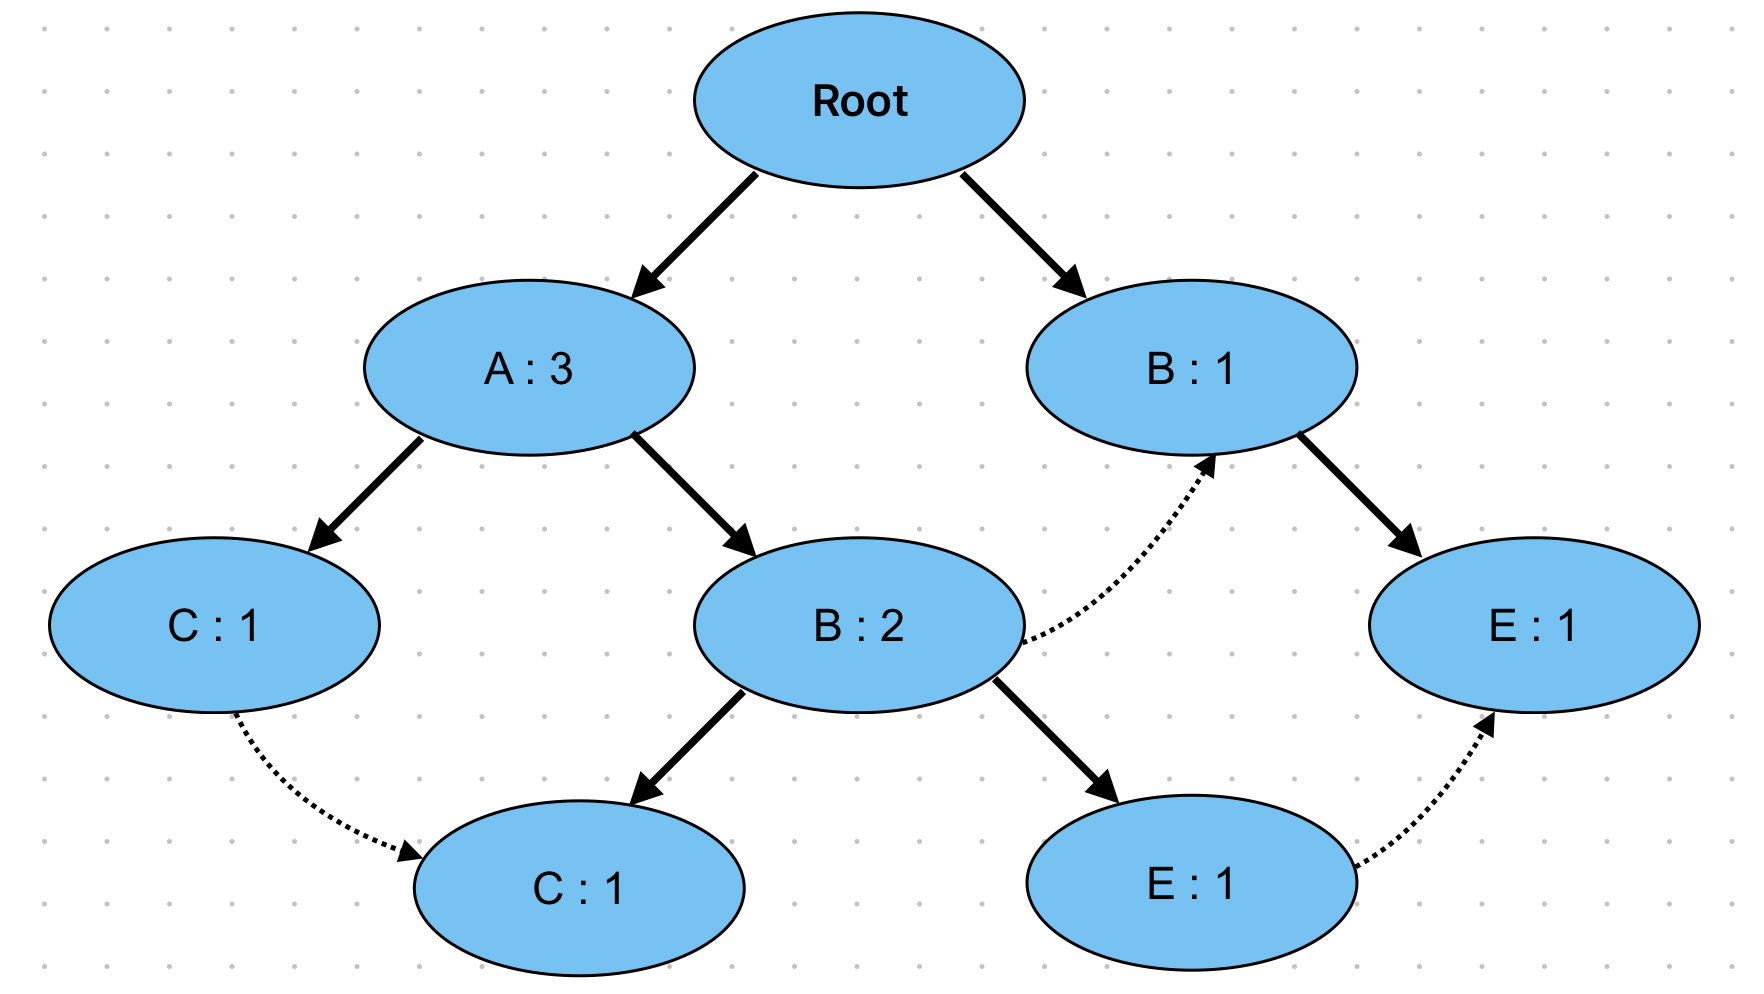
\includegraphics[width=\textwidth]{./images/FPTree2.png}
\end{center}

\section{Clustering}

\subsection*{K-means}

Consider the following eight two-dimensional data points:

\[x_1: (23, 12), x_2: (6, 6), x_3: (15, 0), x_4: (15, 28), x_5: (20, 9),\] 
\[x_6: (8, 9), x_7: (20, 11), x_8: (8,13)\]

Consider k-means algorithm to answer the following questions. You are required to show the information about each final cluster (including the mean of the cluster and all data points in this cluster). You can consider writing a program for this part but you are not required to submit the program.

\begin{enumerate}
    \item If k = 2 and the initial means are (20, 9) and (8, 9), what is the output of the
    algorithm? In the output, you are required to show the information about each final cluster (including the mean of the cluster and all data points in this cluster).
    \item If k = 2 and the initial means are (15, 0) and (15, 29), what is the output of the
    algorithm? In the output, you are required to show the information about each final cluster (including the mean of the cluster and all data points in this cluster).
    \item What are the advantages and the disadvantages of the k-means algorithm? For each disadvantage, please also give a suggestion to enhance the k-means algorithm.
\end{enumerate}

\begin{enumerate}
    \item We first create a table for the data points and their respective distances from the initial means of (20, 9) and (8, 9). We use the Euclidean distance formula to calculate the distance between the data points and the initial means. We then are able to cluster these data points nto k = 2 clusters by finding the smallest distance between the data points and the initial means. We then get the following table:
    
    \begin{table}[h]
        \begin{tabular}{|l|l|l|l|}
        \hline
        K = 2        & d\_1 (20,9) & d\_2 (8,9) & Cluster \\ \hline
        x\_1 (23,12) & 4.24        & 15.30      & 1       \\ \hline
        x\_2 (6,6)   & 14.32       & 3.61       & 2       \\ \hline
        x\_3 (15,0)  & 10.30       & 11.40      & 1       \\ \hline
        x\_4 (15,28) & 19.65       & 20.25      & 1       \\ \hline
        x\_5 (20,9)  & 0.00        & 12.00      & 1       \\ \hline
        x\_6 (8,9)   & 12.00       & 0.00       & 2       \\ \hline
        x\_7 (20,11) & 2.00        & 12.17      & 1       \\ \hline
        x\_8 (8,13)  & 12.65       & 4.00       & 2       \\ \hline
        \end{tabular}
        \centering
    \end{table}

    We then calculate the new means of the clusters by taking the average of the data points in each cluster. We then get the new means of 
    \[C_1 = (\frac{23 + 15 + 15 + 20 + 20}{5}, \frac{12 + 0 + 28 + 9 + 11}{5}) = (18.6,12)\]
    \[C_2 = (\frac{6 + 8 + 8}{3}, \frac{6 + 9 + 13}{3}) = (7.33,9.33)\]

    \item We do the same process as above but with the initial means of (15, 0) and (15, 29). We then get the following table:
    
    \begin{table}[h]
        \begin{tabular}{|l|l|l|l|}
        \hline
        K = 2        & d\_1 (15,0) & d\_2 (15,29) & Cluster \\ \hline
        x\_1 (23,12) & 14.24       & 18.79        & 1       \\ \hline
        x\_2 (6,6)   & 10.82       & 24.70        & 1       \\ \hline
        x\_3 (15,0)  & 0.00        & 29.00        & 1       \\ \hline
        x\_4 (15,28) & 28.00       & 1.00         & 2       \\ \hline
        x\_5 (20,9)  & 10.30       & 20.62        & 1       \\ \hline
        x\_6 (8,9)   & 11.40       & 21.19        & 1       \\ \hline
        x\_7 (20,11) & 12.08       & 18.68        & 1       \\ \hline
        x\_8 (8,13)  & 14.76       & 17.46        & 1       \\ \hline
        \end{tabular}
        \centering
    \end{table}

    We then calculate the new means of the clusters by taking the average of the data points in each cluster. We then get the new means of
    \[C_1 = (\frac{23 + 6 + 15 + 20 + 8 + 20 + 8}{7}, \frac{12 + 6 + 0 + 9 + 9 + 11 + 13}{7})\]
    \[= (14.28,8.57)\]
    \[C_2 = (\frac{15}{1}, \frac{28}{1}) = (15,28)\]

    \item K-Means clustering is a very good algorithm for clustering data points. This is especially true for larger datasets and is very simple as its a simple iterative program. However, it is not always guaranteed to find the optimal solution. This is because the algorithm is dependent on the initial means. If the initial means are not chosen well, the algorithm may not be able to find the optimal solution. One way to enhance the algorithm is to run the algorithm multiple times with different initial means and then choose the solution with the lowest cost function. This way, we can ensure that we are getting the optimal solution. This would also fix the problem of the algorithm not being able to find optimal clusters due to outliers. There also has been problems with K-Mean clustering when there are clusters of different sizes, densities, and being a non-gobular shape. To solve this problem, we can increase the amount of clusters to evenly spread out the data points. 

\end{enumerate}

\subsection*{Hierarchical Clustering}

Consider the following two-dimensional data points:

\begin{table}[h]
    \begin{tabular}{|l|l|l|}
    \hline
    Data point & $x_1$ & $x_2$ \\ \hline
    1          & 0.1   & 0.2   \\ \hline
    2          & 0.2   & 0.1   \\ \hline
    3          & 0.4   & 0.8   \\ \hline
    4          & 0.5   & 1.0   \\ \hline
    5          & 0.7   & 0.35  \\ \hline
    \end{tabular}
    \centering
\end{table}

\begin{enumerate}
    \item Compute the Euclidean distance between every pair of points. Show your results in a 5x5 distance matrix.
    \item Apply the single link (MIN) algorithm to cluster the objects. Draw the dendrogram for the clusters assuming the distance measure is Euclidean. Make sure vou label the distance axis of the dendrogram carefully.
    \item Suppose we apply the complete link (MAX algorithm to cluster the objects.
    Draw the dendrogram for the clusters assuming the distance measure is Euclidean. Make sure you label the distance axis of the dendrogram carefully.
\end{enumerate}

\begin{enumerate}
    \item We first calculate the Euclidean distance between every pair of points. We then get the following distance matrix:
    
    \begin{table}[h]
        \begin{tabular}{|l|l|l|l|l|l|}
        \hline
        DATA POINT & 1   & 2   & 3   & 4   & 5 \\ \hline
        1          & 0   &     &     &     &   \\ \hline
        2          & .14 & 0   &     &     &   \\ \hline
        3          & .67 & .73 & 0   &     &   \\ \hline
        4          & .89 & .95 & .22 & 0   &   \\ \hline
        5          & .62 & .56 & .54 & .68 & 0 \\ \hline
        \end{tabular}
        \centering
    \end{table}

    \item To apply the single link (MIN) algorithm to cluster the objects we have to first find the minimum vaue of the whole table. The first cluster to appear would be the minimum value at points 1 and 2, .14. We then make a cluster of it and shifted every minimum distance. We then get the following table:
    \begin{table}[h]
        \begin{tabular}{|l|l|l|l|l|}
        \hline
        DATA POINT & (1,2) & 3   & 4   & 5 \\ \hline
        (1,2)      & 0     &     &     &   \\ \hline
        3          & .67   & 0   &     &   \\ \hline
        4          & .89   & .22 & 0   &   \\ \hline
        5          & .56   & .54 & .68 & 0 \\ \hline
        \end{tabular}
        \centering
    \end{table}
    The next value is in points 3 and 4 which is the value .22. We then create the cluster and get the following table:

    \begin{table}[h]
        \begin{tabular}{|l|l|l|l|}
        \hline
        DATA POINT & (1,2) & (3,4) & 5         \\ \hline
        (1,2)      & 0     &       & \textbf{} \\ \hline
        (3,4)      & .89   & 0     & \textbf{} \\ \hline
        5          & .56   & .54   & 0         \\ \hline
        \end{tabular}
        \centering
    \end{table}
    
    \newpage

    The last cluster is (3,4) and 5, a value of .54, and after clustering, there is a remaining value of .56. We then get the following table and lastly dendrogram:

    \begin{table}[h]
        \begin{tabular}{|l|l|l|}
        \hline
        DATA POINT & (1,2) & ((3,4),5) \\ \hline
        (1,2)      & 0     &           \\ \hline
        ((3,4),5)  & \textbf{.56}   & 0         \\ \hline
        \end{tabular}
        \centering
    \end{table}

    \begin{center}
    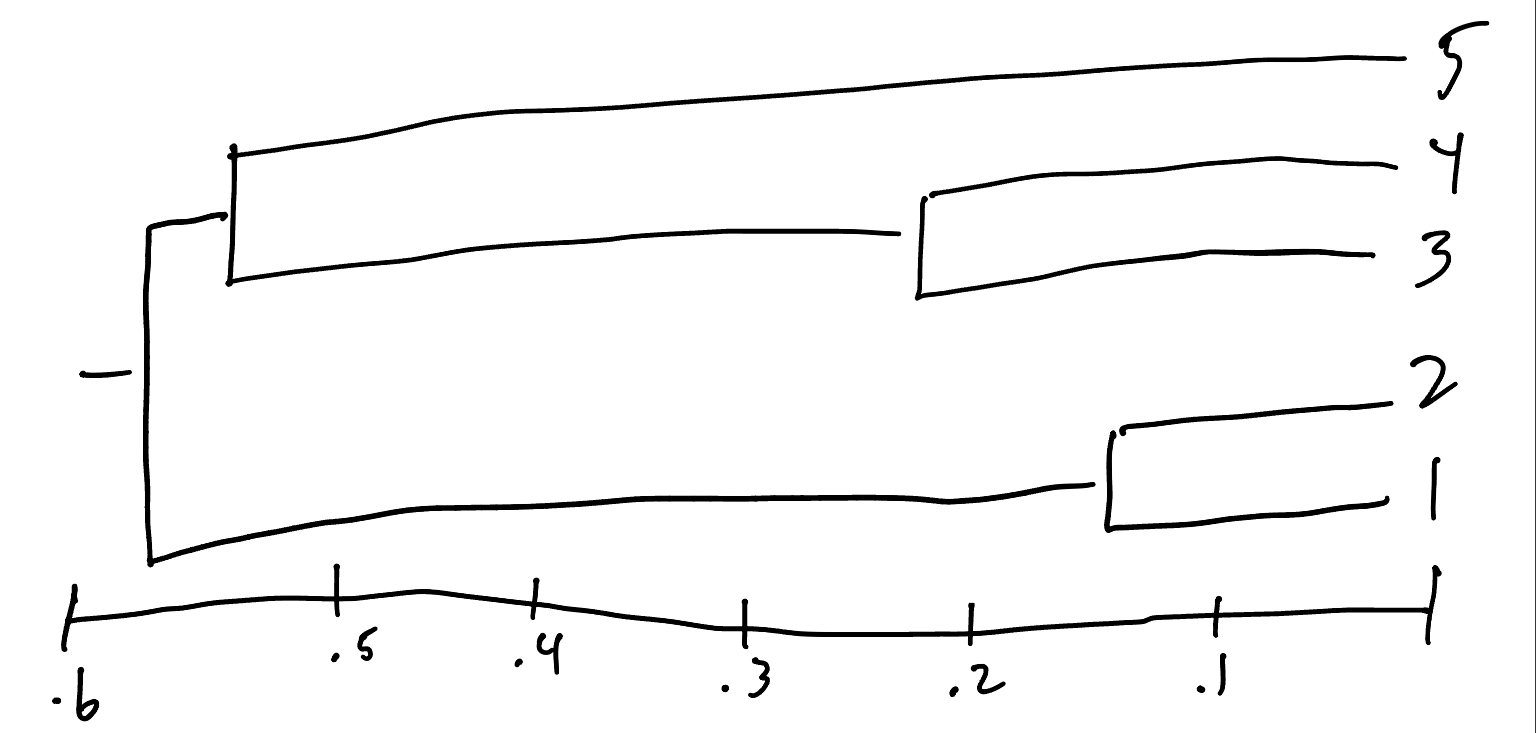
\includegraphics[scale=.2]{./images/Single.jpeg}
    \end{center}

    \item To apply the complete link (MAX) algorithm to cluster the dataset, we do the same as the previous problem, but we use the maximum value instead of the minimum value. We first find the minimum value in the table which in this case would be at points 1 and 4 with the value of .14, then move everything by the maximum instead of the minimum. We then get the following table:
    
    \begin{table}[h]
        \begin{tabular}{|l|l|l|l|l|}
        \hline
        DATA POINT & (1,2) & 3   & 4   & 5 \\ \hline
        (1,2)      & 0     &     &     &   \\ \hline
        3          & .73   & 0   &     &   \\ \hline
        4          & .95   & .22 & 0   &   \\ \hline
        5          & .62   & .54 & .68 & 0 \\ \hline
        \end{tabular}
        \centering
    \end{table}
    
    The next points are 3 and 4 at a value of .22. We then get the following table:

    \begin{table}[h]
        \begin{tabular}{|l|l|l|l|}
        \hline
        DATA POINT & (1,2) & (3,4) & 5 \\ \hline
        (1,2)      & 0     &       &   \\ \hline
        (3,4)      & .95   & 0     &   \\ \hline
        5          & .62   & .68   & 0 \\ \hline
        \end{tabular}
        \centering
    \end{table}

    \newpage

    Lastly we cluster the value .62 at (1,2) and 5 with a remainging value of .95 to get the following table and dendrogram:

    \begin{table}[h]
        \begin{tabular}{|l|l|l|}
        \hline
        DATA POINT & ((1,2),5) & (3,4) \\ \hline
        ((1,2),5)  & 0         &       \\ \hline
        (3,4)      & .95       & 0     \\ \hline
        \end{tabular}
        \centering
    \end{table}

    \begin{center}
        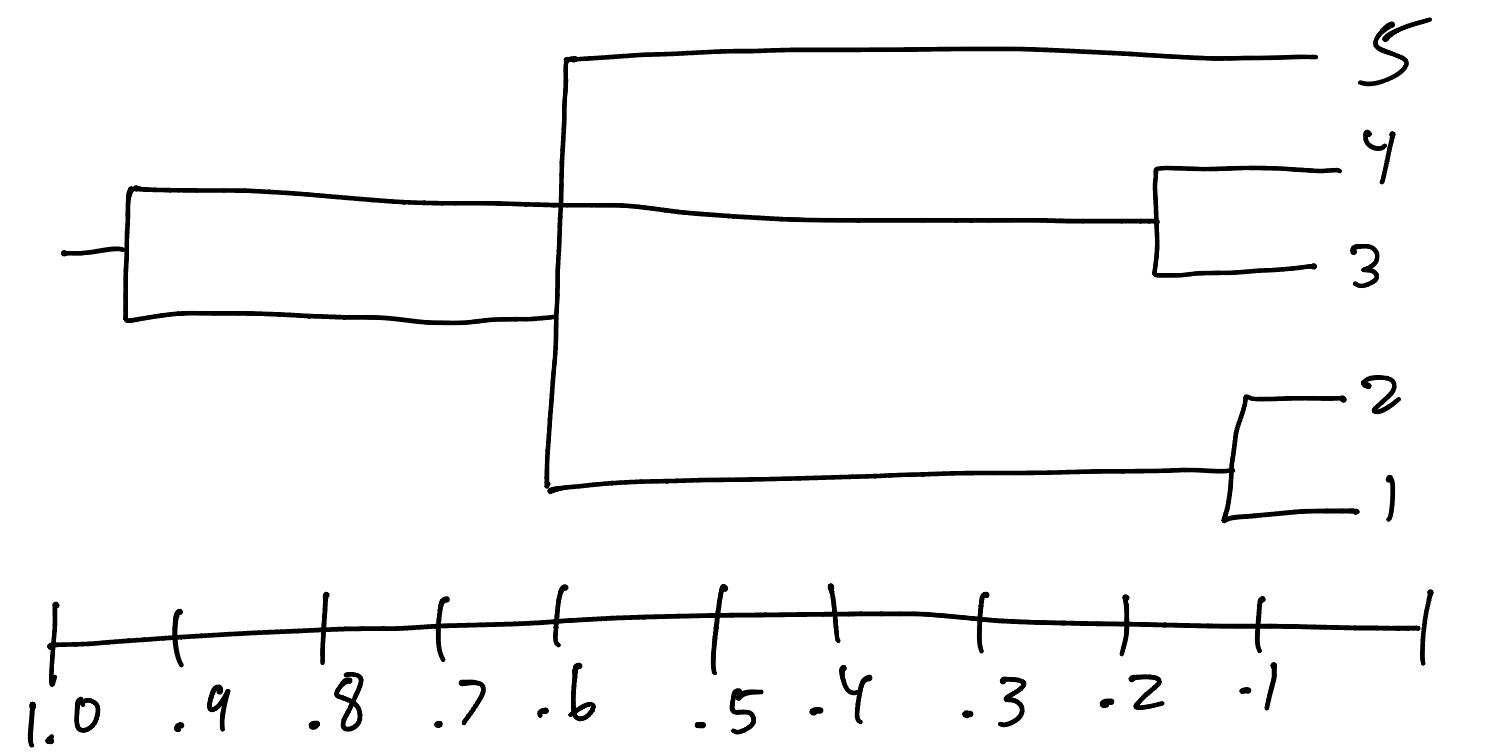
\includegraphics[scale=.21]{./images/Complete.jpeg}
    \end{center}

\end{enumerate}




\end{document}